% Part: sets-functions-relations
% Chapter: relations
% Section: graphs

\documentclass[../../../include/open-logic-section]{subfiles}

\begin{document}

\olfileid{sfr}{rel}{grp}
\olsection{आलेख}

\emph{आलेख} म्हणजे अशी आकृती की जिच्यात ``गाठी'' किंवा ``शिखरे''
(``शिखर'' या शब्दाचे अनेकवचन) म्हटले जाणारे बिंदू कडांनी जोडलेले असतात. विविक्त गणित आणि संगणकशास्त्रात
आलेख सर्वत्र वापरले जातात. विविध जाळ्यांसारख्या ठोस गोष्टींपासून ते
निर्णयांच्या शक्य परिणामांसारख्या अमूर्त संरचनांपर्यंत अनेक संबंध आणि
संरचना दर्शवण्यासाठी व त्यांचे दृश्य रूप देण्यासाठी ते अतिशय उपयोगी
असतात. ग्रंथसाहित्यात आलेखांचे अनेक प्रकार आढळतात. उदाहरणार्थ, कडांना
दिशा आहे की नाही, नावे आहेत की नाहीत, एखाद्या शिखरापासून त्याच शिखरापर्यंत
कड असू शकते की नाही, त्याच शिखरांमध्ये अनेक कडा असू शकतात की नाहीत,
इत्यादी बाबतींत हे प्रकार वेगळे असतात. \emph{दिशित आलेखांचा} संबंधांशी
विशेष संबंध आहे.

\begin{defn}[दिशित आलेख]
\emph{दिशित आलेख} $G = \tuple{V, E}$ म्हणजे \emph{शिखरांचा} $V$ हा संच
आणि \emph{कडांचा} $E \subseteq V^2$ हा संच.
\end{defn}

\begin{explain}
आपल्या व्याख्येनुसार आलेख म्हणजे एक संच आणि त्या संचावरील एक संबंध.
अर्थात, आलेखांबद्दल बोलताना त्यांचे चित्र काढले जावे ही अपेक्षा स्वाभाविक
आहे: $v_1$ आणि $v_2$ ही शिखरे बाणाने तेव्हा आणि केवळ तेव्हाच जोडून
आलेख काढता येतो, जेव्हा $\tuple{v_1, v_2} \in E$.
नुसता संबंध आणि आलेख यांतील फरक एवढाच की आलेखात शिखरांचा संचही स्पष्ट
केलेला असतो, म्हणजे आलेखात एकाकी शिखरे असू शकतात. महत्त्वाचा मुद्दा असा:
$X$ संचावरील प्रत्येक $R$ संबंधाकडे $\tuple{X, R}$ हा दिशित आलेख म्हणून
पाहता येते; आणि उलट, $\tuple{V, E}$ या दिशित आलेखाकडे, $V$ हा संच स्पष्ट
केलेला असताना, $E \subseteq V^2$ हा संबंध म्हणून पाहता येते.
\end{explain}

\begin{ex}
$V = \{1, 2, 3, 4\}$ आणि $E =
\{\tuple{1,1}, \allowbreak \tuple{1, 2}, \allowbreak \tuple{1, 3},
\allowbreak \tuple{2, 3}\}$ असलेला $\tuple{V, E}$ हा आलेख असा दिसतो:
\begin{align*}
& 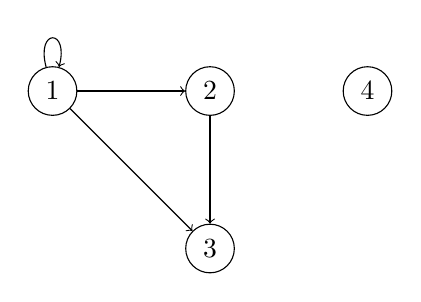
\begin{tikzpicture}[->,node distance=2cm]
  \node[draw,circle] (A) {$1$};
  \node[draw,circle] (B) [right of=A] {$2$};
  \node[draw,circle] (C) [below of=B] {$3$};
  \node[draw,circle] (D) [right of=B] {$4$};
  \draw (A) to [loop above]  (A);
  \draw (A) to  (B);
  \draw (A) to  (C);
  \draw (B) to  (C);
  \end{tikzpicture}
\intertext{हा आलेख $V' = \{1, 2, 3\}$ असणाऱ्या $\tuple{V', E}$ या
  आलेखापेक्षा वेगळा आहे; तो असा दिसतो:}
& 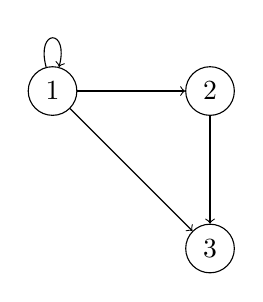
\begin{tikzpicture}[->,node distance=2cm]
  \node[draw,circle] (A) {$1$};
  \node[draw,circle] (B) [right of=A] {$2$};
  \node[draw,circle] (C) [below of=B] {$3$};
  \draw (A) to [loop above]  (A);
  \draw (A) to  (B);
  \draw (A) to  (C);
  \draw (B) to  (C);
  \end{tikzpicture}
\end{align*}
\end{ex}

\begin{prob}
  $\{1, 2, 3, 4\}$ या संचावरील लहान-किंवा-समान असण्याचा $\le$ संबंध
  आलेख म्हणून पाहा आणि त्याची आकृती काढा.
\end{prob}

\end{document}
